\documentclass[10pt,a4paper]{article}
\usepackage[utf8]{inputenc}
\usepackage[english]{babel}
\usepackage{amssymb,amsfonts, amsmath}
\usepackage{graphicx}
\usepackage{listings, color}
\usepackage{url}
\usepackage{float}
\usepackage{hyperref}

\definecolor{dkgreen}{rgb}{0,0.45,0}
\definecolor{gray}{rgb}{0.5,0.5,0.5}
\definecolor{mauve}{rgb}{0.30,0,0.30}

% Default settings for code listings
\lstset{frame=tb,
  aboveskip=3mm,
  belowskip=3mm,
  showstringspaces=false,
  columns=flexible,
  basicstyle={\small\ttfamily},
  numbers=left,
  numberstyle=\footnotesize,
  keywordstyle=\color{dkgreen}\bfseries,
  commentstyle=\color{gray},
  stringstyle=\color{mauve},
  frame=single,
  breaklines=true,
  breakatwhitespace=true,
  tabsize=1
}

\title{\rule{12.5cm}{0.5mm}\\Advanced Algorithms in Computational Biology\\DM845}
\author{Martin Østergaard Villumsen\\\texttt{mvill11@student.sdu.dk}\\\rule{6.5cm}{0.5mm}\\University of Southern Denmark\\}
\date{\today}

\begin{document}
\maketitle
\newpage
\tableofcontents
\newpage
\section{Introduction}
The human genome is diploid which means that each cell has two homologous copies of each chromosome, one from the mother and one from the father. In order to understand the genetic basis for different diseases (e.g. cancer) it is not sufficient to detect the single nucleotide polymorphisms (SNPs), we also need to assign each SNP to the two copies of the chromosome and current methods for doing so suffers from the fact that the reads are too short \cite{whatshap}.

In this project we will develop a simple read simulator, which generates reads that are much longer than those obtained from e.g. Next-Gen sequencing machines. We will simulate reads with different parameters such as read length and sequencing error probability and assign SNPs to each chromosome from these reads using \textsc{WhatsHap}, a novel dynamic programming approach to haplotype assembly described in \cite{whatshap}. We will then evaluate the results and compare them with those presented in \cite{whatshap}.

\subsection{Biological Problem}
The task of assigning SNPs to a concrete chromosome is called phasing and the resulting groups of SNPs are called haplotypes. We need to discover and phase all these SNPs in order to gain a better understanding for e.g. some diseases by linking possibly disease-causing SNPs with one another. By doing so we can reconstruct haplotypes from a collection of sequenced reads which is known as haplotype assembly.

\subsection{Computational Problem}
There are two groups of single nucleotide variants: Those that are homozygous and those that are heterozygous. Individuals that are homozygous at every locus or heterozygous at just one locus can easily be phased, however, if we have $m$ heterozygous SNPs, there are $2^m$ possible haplotypes which illustrates that it is a hard computational problem. Therefore we are only concerned with heterozygous SNPs when doing haplotype assembly. 

What also makes this a computational hard problem is the fact that we want to phase an reconstruct the haplotypes directly from sequencing reads. 

\section{Haplotype Assembly with WhatsHap}
There are two major approaches to phasing variants: One approach relies on genotypes as input along with the zygosity status of the SNPs, and the other approach phases directly from sequencing read data \cite{whatshap}. \textsc{WhatsHap} belongs to the latter. 

\textsc{WhatsHap} has been developed with the parsimony principle in mind, i.e. computing two haplotypes to which we can assign all reads while minimizing the amount of sequencing errors to be corrected or removed \cite{whatshap}. This resembles the minimum error correction (MEC) problem which consists of finding the minimum number of corrections to the SNP values to be made to the input in order to be able to arrange the reads into two haplotypes without conflicts \cite{whatshap}. This can easily be adapted to a weighted version of the problem, namely the weighted minimum error correction problem (wMEC). The weight in this case reflects the relative confidence that a single nucleotide is correctly sequenced.

Even though the wMEC problem is NP-hard \textsc{WhatsHap} creates an exact solution to the problem in linear time. This is done by the use of dynamic programming and assuming a bounded coverage, i.e. the implementation can solve the problem in linear time on datasets of maximum coverage up to 20x \cite{whatshap}. The algorithm is a fixed parameter tractable approach to the wMEC where the running time is only depending on the coverage, i.e. the number of reads that cover a SNP position.

The input to the wMEC problem is a matrix with entries $\in\{0, 1, -\}$ where each row corresponds to a read and each column corresponds to a SNP position. Each entry is associated with a weight telling how likely it is that the entry is correctly sequenced. We want to find a minimum weight solution and when these weights are log-likelihoods, summing them up corresponds to multiplying probabilities, thus finding the minimum weight solution corresponds to finding a maximum likelihood bipartition of the reads \cite{whatshap}. And this is basically what the authors of \textsc{WhatsHap} is using a dynamic programming approach to do. By using this approach they find an optimal solution to the wMEC problem for each column of the matrix and then an optimal bipartition of the reads can be obtained by backtracking along the columns of the dynamic programming table. See \cite{whatshap} for further details.

The implementation of \textsc{WhatsHap} can be found at \url{https://bitbucket.org/whatshap/whatshap} and the documentation can be found at \url{https://whatshap.readthedocs.org/en/latest/}. The software requires a \texttt{VCF}-file and a \texttt{BAM}-file as input. \texttt{VCF}-files describe gene sequence variations, i.e. a list of variants and genotypes for the diploid genome, and \texttt{BAM}-files are the compressed binary equivalent of \texttt{SAM}-files, which are \textit{Sequence Alignment/Map}-files that contain sequence data in a series of tab delimited ASCII columns, i.e. aligned reads for the individual diploid genome that are coordinate sorted (i.e. by chromosal position).
% Description of data

\section{Building a DNA Simulator}
There already exists different DNA read simulators but for this project we decided to design and implement our own simple simulator to generate data for \textsc{WhatsHap}. The lecturer of the course has provided a reference chromosome (\texttt{chr1.fa}) which we have used as a basis for the simulation of DNA reads. The chromosome is in \texttt{FASTA}-format (\texttt{.fa}) which is a text-based format for representing nucleotide sequences.

For this implementation we have used \texttt{Python 2.7.9}. Also, for this implementation we assume that there are no \texttt{N}s in the chromosome, i.e. the \texttt{N}s present in \texttt{chr1.fa} are removed and the only letters present are: \texttt{A, T, C, G}.

\subsection{Generating a Chromosome with Mutations}
Before building the actual simulator we needed a script to generate a \texttt{VCF}-file describing the chromosome with mutations. Generating the \texttt{VCF}-file is done with a simple \texttt{Python} script that reads the chromosome, removes all \texttt{N}s (if there are any) and copy the chromosome one nucleotide at a time. Every 400 + 'random integer between 0-100' we simulate a mutation (i.e. a single nucleotide variant) by randomly choosing one of the remaining nucleotides. E.g. if the current nucleotide is \texttt{A} we randomly choose a nucleotide from \{\texttt{T, C, G}\}. For every simulated mutation a line is written to the \texttt{VCF}-file with the following values:
\begin{itemize}
\item CHROM: \texttt{'chr1'}
\item POS: The position of the nucleotide in the chromosome
\item ID: The position of the nucleotide in the chromosome
\item REF: The nucleotide from the reference chromosome
\item ALT: The "new" nucleotide (i.e. the variant)
\item QUAL: \texttt{'.'}
\item FILTER: \texttt{'PASS'}
\item INFO: \texttt{'.'}
\item FORMAT: \texttt{'GT'}
\item sample: \texttt{'0/1'}
\end{itemize}
These values were primarily chosen based on miscellaneous testdata for \textsc{WhatsHap}.

This \texttt{VCF}-file can then be used to generate a copy of the chromosome with mutations which we will need for simulating the DNA reads.

See \texttt{buildVCF.py} for details on the implementation.

\subsection{Simulating DNA Reads}
There are two types of variants which can occur in DNA reads: Sequencing errors and mutations. We need to take both into account when designing a read simulator. Also, we need to be able to choose how many reads the simulator should generate, how long the reads should be and the percentage of sequencing errors that should occur in the simulated reads. This is all given as parameters to the program. We have designed the read simulator as follows:
\begin{enumerate}
\item Read the \texttt{FASTA}-file (reference chromosome) and the \texttt{VCF}-file (both are given as input) and remove line breaks, comments etc.
\item Generate a copy of the reference chromosome with mutation from the \texttt{VCF}-file.
\item Generate reads one at a time as follows:
\subitem a. Choose one of the two chromosomes at random.
\subitem b. Choose a random start position for the read.
\subitem c. Iterate over the next $x$ nucleotides, where $x$ is the read length.
\subitem d. For each nucleotide in the read, alter the nucleotide with probability $e$, where $e$ is the probability that a sequencing error occurs.
\item Repeat a. - d.  $r$ times where $r$ is the number of reads we want to generate.
\end{enumerate}
When all reads have been generated the program generates a \texttt{SAM}-file describing the reads, which is written to a file. We have chosen to leave out many of the values of the \texttt{SAM}-file to keep things simple. We have chosen to use the following header:
\begin{lstlisting}
@HD	VN:1.4	GO:none	SO:coordinate
@SQ	SN:chr1	LN:'length of chromosome'
@RG	ID:1	PL:Platform	LB:library	SM:sample
\end{lstlisting}
along with the following values for each line of the file:
\begin{itemize}
\item QNAME: \texttt{'r00\%d'} where '\%d' is the start position of the read in the reference chromosome
\item FLAG: \texttt{'0'}
\item RNAME: \texttt{'chr1'}
\item POS: 'Start position of the read in the reference chromosome'
\item MAPQ: '255' (this indicates that the value is not available)
\item CIGAR: \texttt{'\%dM'} where '\%d' is the length of the read
\item RNEXT: \texttt{'='}
\item PNEXT: \texttt{'0'}
\item TLEN: 'Length of the chromosome'
\item SEQ: 'The actual read'
\item QUAL: 'A string of length $r$ consisting of "J"s, where $r$ is the length of the read'
\end{itemize} 
These values were primarily chosen based on miscellaneous testdata for \textsc{WhatsHap}.

For details about the individual field see the SAM Format Specification at \url{https://samtools.github.io/hts-specs/SAMv1.pdf}. For details about the implementation of the simulator see \texttt{sim.py}.

\subsection{Using the Simulator}
In order use the simulator that is described above we first need to simulate a \texttt{VCF}-file describing a mutated version of the reference chromosome. As mentioned earlier we have used chromosome 1 (\texttt{chr1.fa}) for reference chromosome. The script to generate a \texttt{VCF}-file is run with the following command:
\begin{lstlisting}
python buildVCF.py chr1.fa chr1.vcf
\end{lstlisting}
where \texttt{chr1.vcf} is the file that will be generated by the script. \texttt{chr1.vcf} can then be used for simulating the DNA read data. This is done with the following command:
\begin{lstlisting}
python sim.py chr1.fa chr1.vcf numberReads readLength errorProb chr1.sam
\end{lstlisting}
where \texttt{numberReads} and \texttt{readLength} are integers stating the number of reads to simulate and the length of the reads respectively. \texttt{errorProb} is a float and states the sequencing error probability and \texttt{chr1.sam} is the sequence alignment/map file that will be generated which describes the simulated reads.

In order to run \textsc{WhatsHap} on the simulated data we need to convert the \texttt{SAM}-files to their binary equivalent \texttt{BAM}-files. This is done by the use of \texttt{samtools}\footnote{See \url{http://www.htslib.org/} for more information about \texttt{samtools}} and a small shell script:
\begin{lstlisting}
for f in *.sam; do samtools view -bS $f | samtools sort - ${f\%.sam}.sorted; done
\end{lstlisting}
which convert and sort every \texttt{SAM}-file in a folder and output their equivalent \texttt{BAM}-files as \texttt{filename.sorted.bam}, where \texttt{filename} is the filename of the input \texttt{SAM}-file. The output \texttt{BAM}-files can then be used as input to \textsc{WhatsHap} along with the generated \texttt{VCF}-file (\texttt{chr1.vcf}).

\subsection{Phasing the Simulated Data}
In order to phase the simulated data we ran \textsc{WhatsHap} with the following command:
\begin{lstlisting}
python3 -m whatshap --ignore-read-groups chr1.vcf chr1.sorted.bam > phased.vcf
\end{lstlisting}
where \texttt{chr1.vcf} and \texttt{chr1.sorted.bam} are the input files which were generated with \texttt{buildVCF.py} and \texttt{sim.py} and \texttt{phased.vcf} is the output file describing the SNPs and what chromosome each variant belongs to.

\section{Results and Discussion}
\textsc{WhatsHap} has been developed with future generation of sequencing machines in mind which generates much longer reads than then currently used technologies such as NextGen. Current technologies generate reads of $\approx$ 150bp - 250bp while future generation sequencing machines generate reads of $\approx$ 1000bp, however, the sequencing error rate is also higher than the currently used technologies. We have therefore chosen to simulate data with the following parameters:
\begin{itemize}
\item Number of reads:
\subitem 100.000
\subitem 500.000
\subitem 1.000.000
\item Read length:
\subitem 500
\subitem 1000
\subitem 1500
\item Error rate:
\subitem 5\%
\subitem 10\%
\subitem 15\%
\end{itemize}
Giving us a total of 27 simulations which we have phased using \textsc{WhatsHap}, however we have only been able to phase 15 of those simulations. When trying to phase the remaining 12 simulations with \textsc{WhatsHap} we received the following assertion error when trying to read the \texttt{BAM}-file given as input:
\begin{lstlisting}
File "/home/martin_15/.local/lib/python3.4/site-packages/whatshap/ scripts/whatshap.py", line 153, in read
    assert 0 < len(readlist) <= 2
AssertionError
\end{lstlisting}
and after digging into the source code of \textsc{WhatsHap} (more specifically \texttt{whatshap.py} line 153) it seems that the error was caused by the fact that none of the simulated reads cover at least one variant. Also, the 12 simulations that we were unable to phase included all simulations with 1.000.000 reads and 3 with 500.000 reads, so it seems that the more reads the more likely it is that the assertion error arise. We suspect that this is due to some error in the implementation of our read simulator but we have not been able to determine the concrete problem.

\subsection{Results}
In order to evaluate the results of the phasings we were able to do we made a small \texttt{Python} script to compare the \texttt{'sample'}-value (i.e. the value stating which chromosome the SNPs belongs to, e.g. \texttt{'0/1'}) of the \texttt{chr1.vcf}-file and the output \texttt{VCF}-files from \textsc{WhatsHap} and counting matches and mismatches in order to calculate the percentage of correctly phased SNPs. This script was called with the following command:
\begin{lstlisting}
python evaluate.py chr1.vcf phased.vcf
\end{lstlisting}
where \texttt{chr1.vcf} is the file generated by \texttt{buildVCF.py} and \texttt{phased.vcf} is the output file from \textsc{WhatsHap}. For details of the implementation see \texttt{evaluate.py}.

The results have been plotted using an \texttt{R}-script\footnote{Implemented in \texttt{results.R}} and the percentage of correctly phased SNPs is illustrated in \hyperref[fig:100k]{Figure 1} for 100.000 reads and and \hyperref[fig:500k]{Figure 2} for 500.000 reads. As we can see on the two plots it seems that the shorter the reads the more matches are obtained and also the percentage of matches is a bit higher if we use 100.000 reads instead of 500.000 reads. This seems a bit odd since \textsc{WhatsHap} have been developed for longer reads. However, the error rate does not seem to influence the number of matches by much.

We have also made two plots illustrating the performance of the phasing in terms of the percentage of unphasable positions versus the error rate. \hyperref[fig:unphasable100k]{Figure 3} illustrates the performance of phasing for 100.000 reads and  \hyperref[fig:unphasable500k]{Figure 4} shows the same plot for 500.000 reads. These two plots clearly shows that the length of the reads have a great influence on the amount of unphasable positions and comparing \hyperref[fig:unphasable100k]{Figure 3} and \hyperref[fig:unphasable500k]{Figure 4} with Fig. 2 in \cite{whatshap} we achieve somewhat similar results that show that the reads of length 1000 and 1500 have a lot lower percentage of unphasable positions than the reads of length 500. Also, the percentage of unphasable reads seems to increase slightly with the error rate but the increase is so small that it seems to be irrelevant.

\subsection{Time and Memory Performance}
One of the advantages of \textsc{WhatsHap} is the low memory and time usage, e.g. as mentioned in \cite{whatshap} the software can solve any problem instance with 15x coverage in less than 10 minutes on a single core CPU. Therefore we have also measured the memory and time usage of \textsc{WhatsHap} for the different parameters of our simulations. This was done using \texttt{/usr/bin/time} in the shell with the following command:
\begin{lstlisting}
/usr/bin/time -v -o outputFile.txt python3 -m whatshap --ignore-read-groups chr1.vcf chr1.sorted.bam > chr1.out.vcf
\end{lstlisting}
which saves all memory and time usage in \texttt{outputFile.txt}. We have plotted all the results obtained from measuring the memory and time usage of the phasing for all our simulations. Looking at the measurements the error rate did not seem to have any significant influence on the memory and time usage so we have chosen to take the average of the measurements with the same number of reads and read length and used these average measurements for the plot.

The results are illustrated in \hyperref[fig:performance]{Figure 5} which shows that even for the most time and memory consuming dataset (500.000 reads and reads of length 1500) \textsc{WhatsHap} only used approximately 3 minutes and 1.2GB of memory. The plot illustrates that the increase in time and memory usage seems to be growing linearly with the length of the reads and also that the number of reads has a great influence on the time and memory usage which seems quite obvious.

\section{Conclusion}
Haplotype assembly and phasing SNPs is important in terms of understanding, diagnosing and treating diseases such as cancer. \textsc{WhatsHap} is one tool among many for haplotype assembly, however, it is the first to solve the weighted minimum error correction problem with long reads to optimality in practice \cite{whatshap}.

The purpose of this project was to develop a simple DNA read simulator to simulate long reads and use \textsc{WhatsHap} to phase the simulated data. We have developed and implemented a DNA read simulator which seems to be working and produce fairly acceptable results, however, when generating $\geq$ 500.000 reads the simulator produces reads where none of the reads seems to be covering any variants. At least that is why \textsc{WhatsHap} is failing and we have not been able to determine the concrete cause of this problem.

We simulated reads with a mixture of three different number of reads, length of reads and error rate, i.e. a total of 27 simulations, of which we were able to phase 15 simulations with \textsc{WhatsHap}.

The results of the haplotype assembly with the simulated data seems to agree somewhat with the results presented in \cite{whatshap} (See \hyperref[fig:unphasable100k]{Figure 3} and \hyperref[fig:unphasable500k]{4}) although the percentage of correctly phased SNPs in general seems to be a bit low with the simulated data compared to what is presented in \cite{whatshap}. So it seems that \textsc{WhatsHap} is a very efficient tool for haplotype assembly for long reads and even though we were unable to run \textsc{WhatsHap} on the vast amount of simulated reads (i.e. $\geq$ 500.000) we still managed to obtain results that agree somewhat with those presented in \cite{whatshap}.

\newpage
\addcontentsline{toc}{section}{References}
\bibliography{whatshap}{}
\bibliographystyle{abbrv}
\newpage
\appendix
\section{Figures}
\begin{figure}[!ht]
\centering
\label{fig:100k}
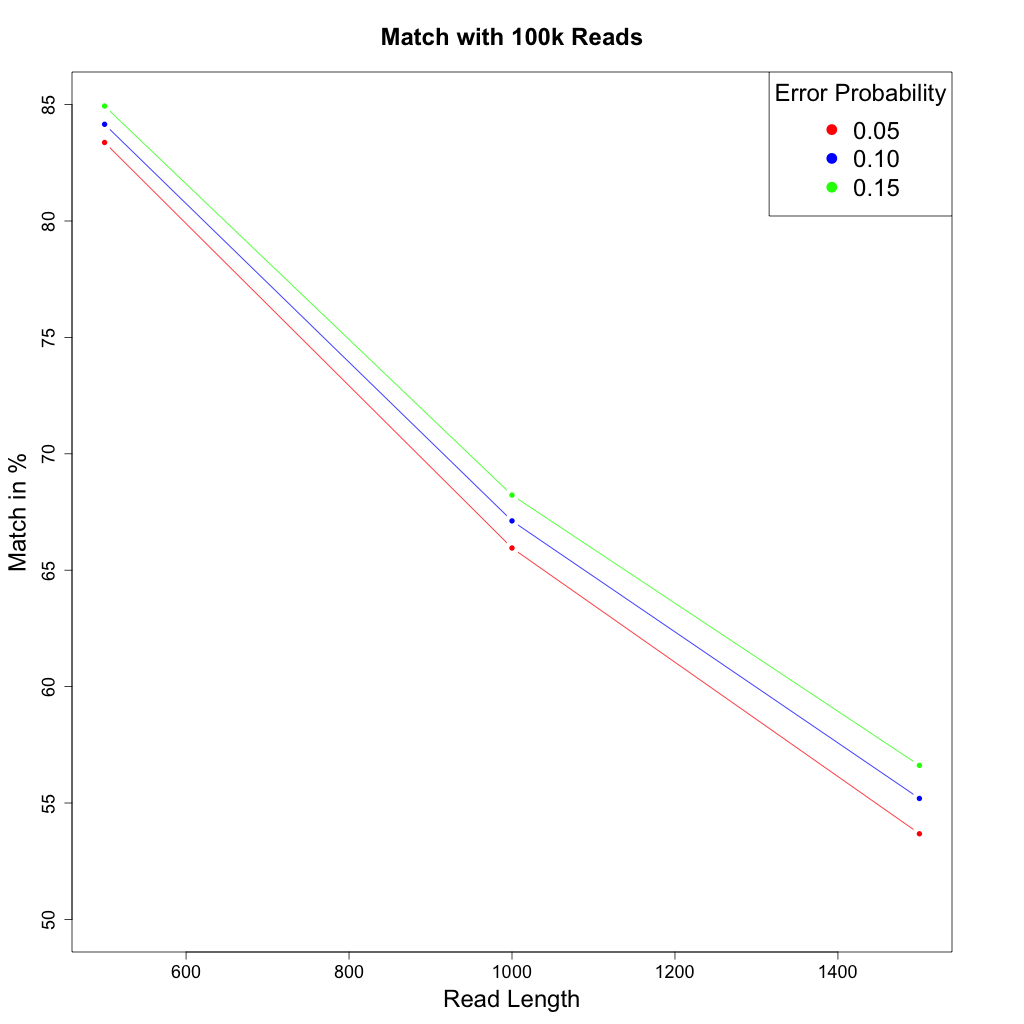
\includegraphics[height=0.43\textheight]{../output/plots/plot100k}
\caption{\footnotesize Results of haplotype assembly of 100.000 reads.}
\label{fig:500k}
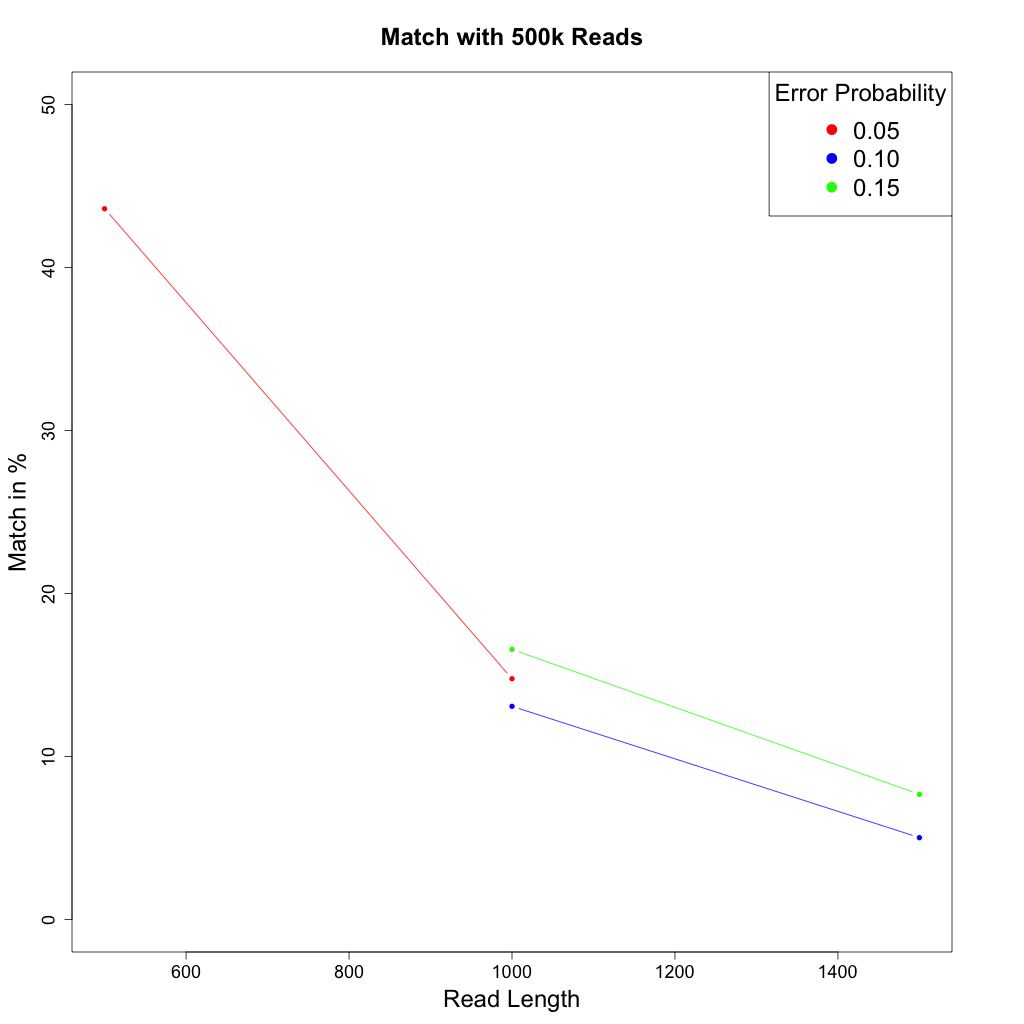
\includegraphics[height=0.43\textheight]{../output/plots/plot500k}
\caption{\footnotesize Results of haplotype assembly of 500.000 reads.}
\end{figure}
\newpage
\begin{figure}[!ht]
\centering
\label{fig:unphasable100k}
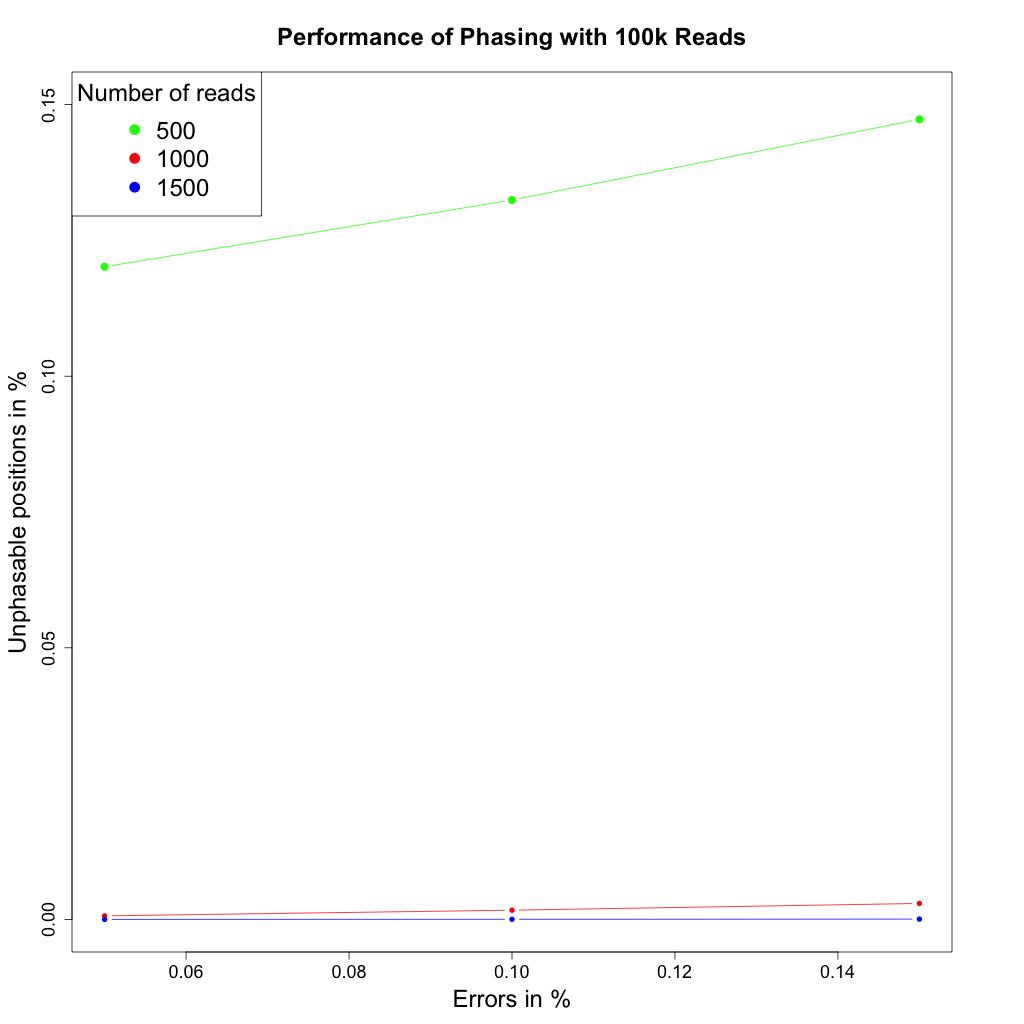
\includegraphics[height=0.5\textheight]{../output/plots/unphasable100k}
\caption{\footnotesize Performance of phasing with 100.000 reads.}
\label{fig:unphasable500k}
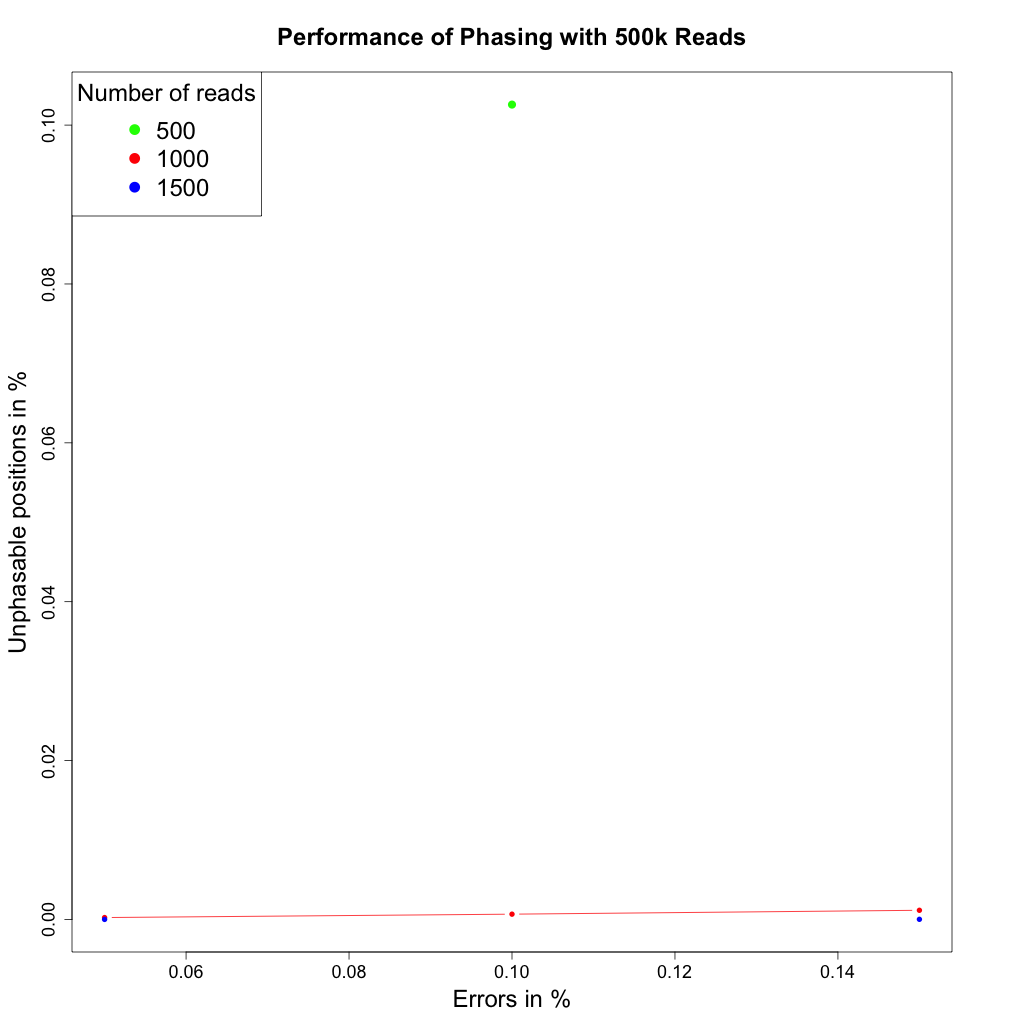
\includegraphics[height=0.5\textheight]{../output/plots/unphasable500k}
\caption{\footnotesize Performance of phasing with 500.000 reads.}
\end{figure}
\newpage
\begin{figure}[!ht]
\centering
\label{fig:performance}
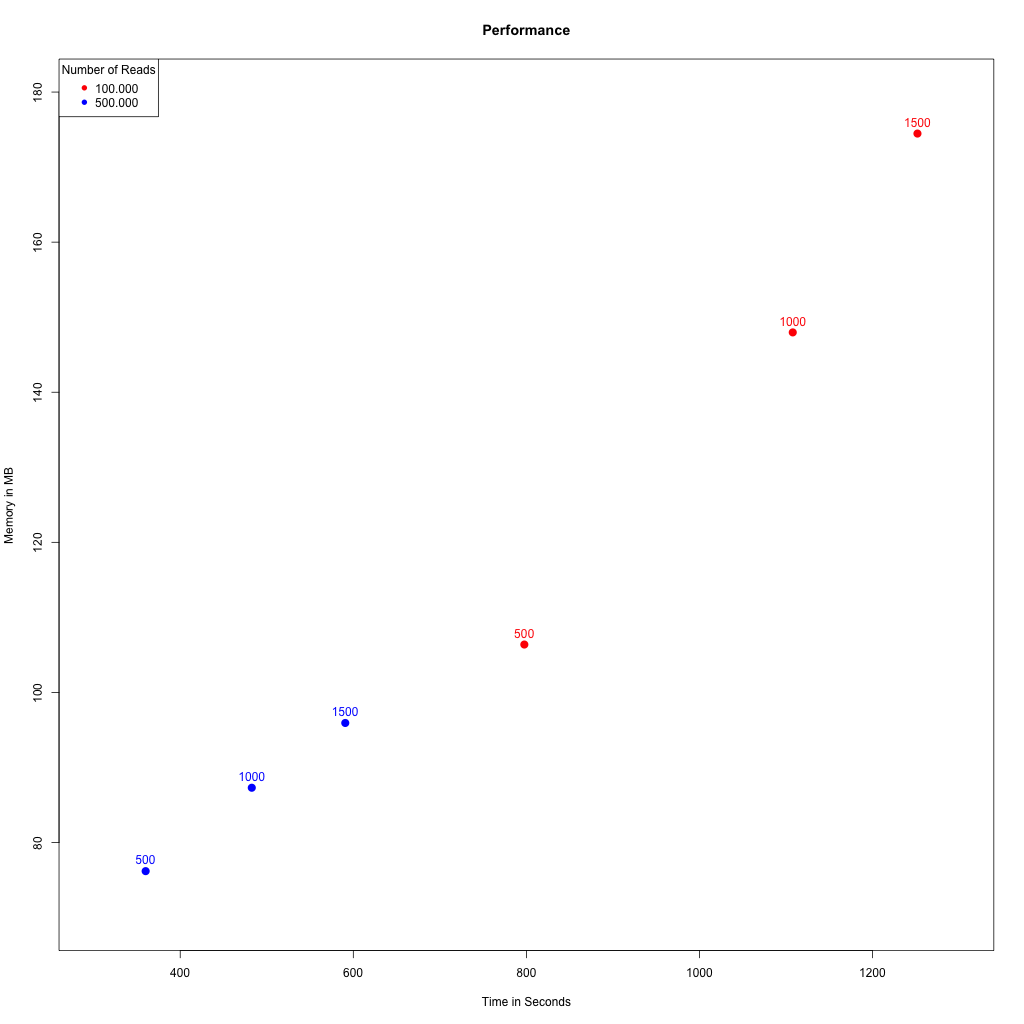
\includegraphics[width=\textwidth]{../output/plots/plotPerformance}
\caption{\footnotesize Performance measured in memory (in MB) and time (in sec.) and with two different number of reads. The numbers above each point indicates the length of the reads.}
\end{figure}

\end{document}
